\section{Current System}

%Disposition
%kort introduction til hvad det er
%scenarier hvor bycyklen kan bruges
%hvem vedligeholder det
%cyklernes placering
%Positive erfaringer med bycyklen, ref god kilde

\bycykel is a bicycle system where citizens in Aalborg are able to borrow bicycles to travel around the city.
The system was started in September 2008 as part of the CIVITAS ARCHIMEDES project, which focuses on making bicycles more widely used \citep{misc:aalborgcykling}.
The bicycles can be found in stations located around the city of Aalborg, see \figref{fig:CykelLokationer}.

\begin{figure}
	\centering
	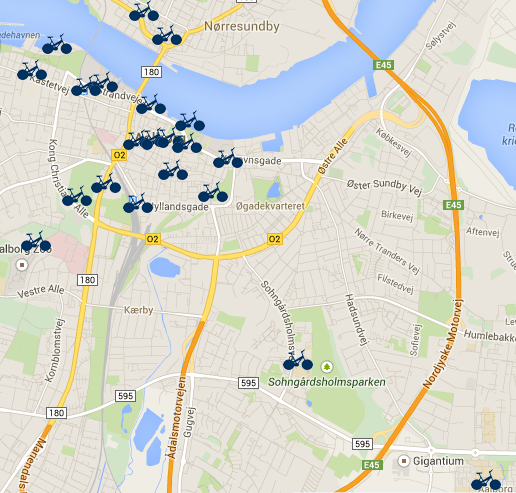
\includegraphics{analysis/CykelLokationer}
	\caption{Bicycle locations \citep{misc:aalborgbycykel}.}
	\label{fig:CykelLokationer}
\end{figure}

As can be seen, the bicycles are mostly located in the center of Aalborg, whereas fewer are placed in other areas.
This means it is easier to borrow and return a bicycle in the central area.

In 2009, 135 bicycles was placed in Aalborg, whereas in 2012 this number had been increased to 200 bicycles \citep{misc:aalborgcykling}.

In order to borrow a bicycle, you need to go to one of the bicycle stations, deposit 20 DKK to unlock the bicycle, then return it to a station when you have no further need of the bicycle \citep{misc:aalborgbycykelregler}, where you will then retrieve your 20 DKK, which makes the system free to use.
This system is built on trust, as if everyone would not return the bicycles to their stations when finished using them, the bicycles would gradually disappear.

\bycykel has had, as of 2012, success with their system. According to a report, if there had not been bicycles more than half of the users would have walked and 5 percent would have driven in a car instead \citep{misc:aalborgcykling}.
Furthermore, it shows that over three season the percentage of bicycles lost has been on maximum 11 percent \citep{misc:aalborgcykling}.

As the bicycles are borrowed by depositing 20 DKK, it means that there is no additional monitoring of where the bicycles are located around the city, other than travelling around the city to locate the bicycles.
This poses the problem that it can be difficult for Aalborg Kommune and the citizens to know which stations have bicycles.
Another problem is if the bicycles are not returned to their stations after use, Aalborg Kommune has difficulty locating such misplaced bicycles.

On their website, it shows that a way for them of locating misplaced bicycles is through citizens reporting lost bicycles by way of SMS and voice mail, or by returning the bicycle themselves claiming the 20 DKK \citep{misc:aalborgbycykelmangler}.
However, if a lost bicycle is not reported or returned by a citizen, the bicycle is practically lost.
The company AFA JCDecaux is in charge of bicycle maintenance and storage during winter time and is also the company in charge of locating the lost bicycles \citep{misc:aalborgcykling}.


These problems could possibly be resolved, and to find inspiration to a solution, other existing systems are analysed hereafter.